% =============================================================================
%  SECTION 2 — INTRIGUING PROPERTIES OF LARGE LANGUAGE MODELS
%  In-Context Learning, Mesa-Optimizers, OPRO, and The Reversal Curse
%  30-minute presentation for executive education
% =============================================================================
\documentclass[aspectratio=169, 12pt]{beamer}

% --- Theme -------------------------------------------------------------------
\usetheme{metropolis}
\usepackage{appendixnumberbeamer}

% --- Packages ----------------------------------------------------------------
\usepackage[T1]{fontenc}
\usepackage{lmodern}
\usepackage{amsmath, amssymb}
\usepackage{tikz}
\usetikzlibrary{arrows.meta, positioning, calc, decorations.pathmorphing,
                 shapes.geometric, fit, backgrounds, matrix}
\usepackage{pgfplots}
\pgfplotsset{compat=1.18}
\usepackage{booktabs}
\usepackage{xcolor}

% --- Custom colours ----------------------------------------------------------
\definecolor{anthblue}{HTML}{1B1F3B}
\definecolor{anthcyan}{HTML}{00B4D8}
\definecolor{anthorange}{HTML}{E07A5F}
\definecolor{anthgreen}{HTML}{81B29A}
\definecolor{lightgray}{HTML}{F0F0F0}
\definecolor{deepred}{HTML}{C1292E}

\setbeamercolor{frametitle}{bg=anthblue, fg=white}
\setbeamercolor{progress bar}{fg=anthcyan}
\setbeamercolor{alerted text}{fg=anthorange}

% --- Metadata ----------------------------------------------------------------
\title{Intriguing Properties of\\Large Language Models}
\subtitle{In-Context Learning, Mesa-Optimizers, and the Reversal Curse}
\author{Executive Education in AI \& Business}
\date{2026}
\institute{}

% =============================================================================
\begin{document}

% --- Title Slide -------------------------------------------------------------
\begin{frame}[plain]
  \titlepage
  \note{Welcome. Today we go deep into two phenomena that reveal something
    fundamental about how large language models work --- and fail.  First:
    they contain their own learning algorithm.  Second: their knowledge is
    stored in a way no human brain would tolerate.}
\end{frame}

% --- Session Map -------------------------------------------------------------
\begin{frame}{Roadmap}
  \begin{center}
  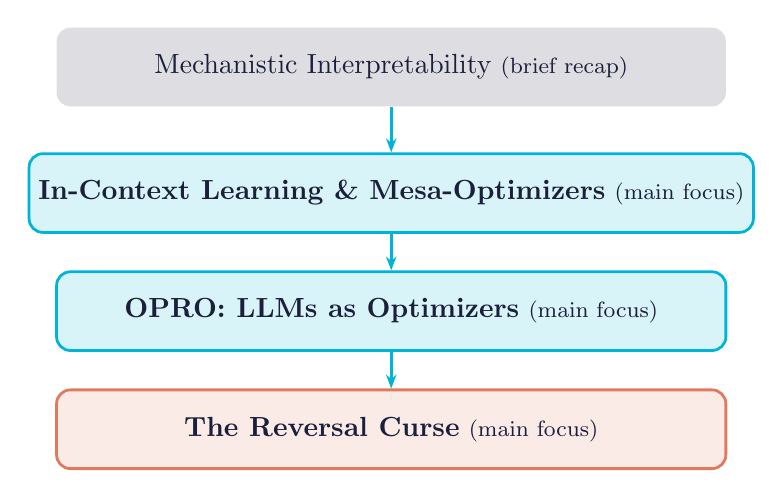
\begin{tikzpicture}[
    block/.style={rounded corners=5pt, minimum width=8.5cm,
                  minimum height=1cm, align=center, font=\normalsize},
    arr/.style={-{Stealth[length=5pt]}, line width=1.2pt, anthcyan},
    dim/.style={font=\footnotesize\itshape, text=anthblue!50}
  ]
    \node[block, fill=anthblue!15, text=anthblue] (A) at (0, 3.6)
      {Mechanistic Interpretability \hfill{\footnotesize(brief recap)}};
    \node[block, fill=anthcyan!15, text=anthblue,
          draw=anthcyan, line width=1pt] (B) at (0, 2.0)
      {\textbf{In-Context Learning \& Mesa-Optimizers}
       \hfill{\footnotesize(main focus)}};
    \node[block, fill=anthcyan!15, text=anthblue,
          draw=anthcyan, line width=1pt] (B2) at (0, 0.5)
      {\textbf{OPRO: LLMs as Optimizers}
       \hfill{\footnotesize(main focus)}};
    \node[block, fill=anthorange!15, text=anthblue,
          draw=anthorange, line width=1pt] (C) at (0, -1.0)
      {\textbf{The Reversal Curse} \hfill{\footnotesize(main focus)}};
    \draw[arr] (A.south) -- (B.north);
    \draw[arr] (B.south) -- (B2.north);
    \draw[arr] (B2.south) -- (C.north);
  \end{tikzpicture}
  \end{center}
  \note{A quick recap of interpretability to set the stage, then the bulk
    of our time on two deep dives: in-context learning (including OPRO,
    where the LLM literally becomes an optimizer) and the reversal curse.}
\end{frame}

% =============================================================================
% BRIEF RECAP — MECHANISTIC INTERPRETABILITY
% =============================================================================

\begin{frame}{Recap: We Can Now See Inside}
  \begin{columns}[c]
    \column{0.55\textwidth}
    \begin{itemize}
      \setlength\itemsep{10pt}
      \item Individual neurons are \alert{polysemantic}\\
        {\small (one neuron $\to$ many concepts)}
      \item Concepts $=$ \textbf{directions} in activation space\\
        {\small packed via \emph{superposition}}
      \item Sparse autoencoders decompose\\
        activations into interpretable features\\
        {\small (34M features from Claude 3 Sonnet)}
      \item Circuit tracing reveals multi-hop\\
        reasoning chains inside the model
    \end{itemize}

    \column{0.42\textwidth}
    \begin{center}
    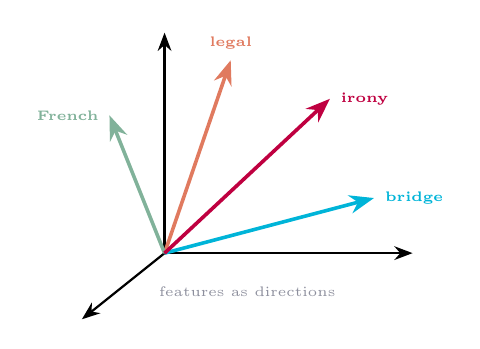
\begin{tikzpicture}[scale=0.7]
      \draw[-{Stealth}, thick] (0,0) -- (4.5,0);
      \draw[-{Stealth}, thick] (0,0) -- (0,4);
      \draw[-{Stealth}, thick] (0,0) -- (-1.5,-1.2);
      \draw[-{Stealth}, anthcyan, line width=1.3pt]
        (0,0) -- (3.8, 1) node[right, font=\tiny\bfseries] {bridge};
      \draw[-{Stealth}, anthorange, line width=1.3pt]
        (0,0) -- (1.2, 3.5) node[above, font=\tiny\bfseries] {legal};
      \draw[-{Stealth}, anthgreen, line width=1.3pt]
        (0,0) -- (-1, 2.5) node[left, font=\tiny\bfseries] {French};
      \draw[-{Stealth}, purple, line width=1.3pt]
        (0,0) -- (3, 2.8) node[right, font=\tiny\bfseries] {irony};
      \node[font=\tiny, text=anthblue!50] at (1.5, -0.7)
        {features as directions};
    \end{tikzpicture}
    \end{center}
  \end{columns}

  \vspace{0.3cm}
  {\footnotesize
    Elhage et al., ``Toy Models of Superposition,'' 2022. \quad
    Templeton et al., ``Scaling Monosemanticity,'' Anthropic, May 2024.}

  \note{Quick recap from last time.  Neural networks are no longer black
    boxes.  Individual neurons are meaningless, but directions in
    activation space correspond to human-understandable concepts.  We can
    extract them, label them, and even manipulate them.  Now: what happens
    when we look at the \emph{computation} the model performs?}
\end{frame}

% =============================================================================
% PART 1 — IN-CONTEXT LEARNING
% =============================================================================

\begin{frame}[standout]
  \Large Part I\\[8pt]
  \normalsize In-Context Learning\\[4pt]
  {\small\itshape The model that learned to learn}
\end{frame}

% --- The Phenomenon ----------------------------------------------------------
\begin{frame}{The Puzzle of In-Context Learning}
  \begin{center}
  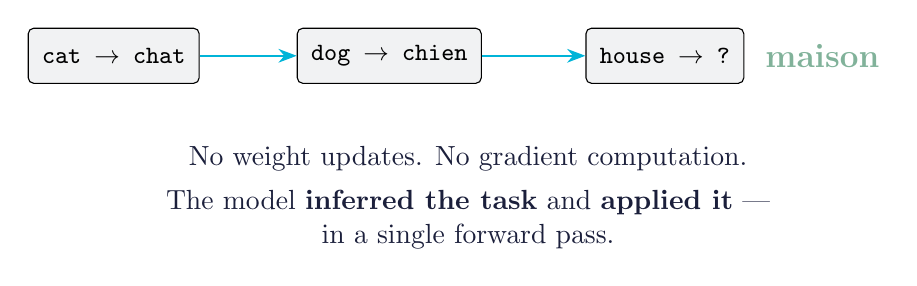
\begin{tikzpicture}[
    tok/.style={draw, rounded corners=2pt, minimum height=0.7cm,
                font=\small, inner sep=5pt, fill=anthblue!6}
  ]
    \node[tok] (e1) at (0, 2) {\texttt{cat $\to$ chat}};
    \node[tok] (e2) at (3.5, 2) {\texttt{dog $\to$ chien}};
    \node[tok] (e3) at (7, 2) {\texttt{house $\to$ ?}};

    \draw[-{Stealth}, anthcyan, thick] (e1.east) -- (e2.west);
    \draw[-{Stealth}, anthcyan, thick] (e2.east) -- (e3.west);

    \node[font=\large\bfseries, anthgreen] at (9, 2) {maison};

    \node[font=\normalsize, text=anthblue, align=center] at (4.5, 0.2) {
      No weight updates.  No gradient computation.\\[4pt]
      The model \textbf{inferred the task} and \textbf{applied it} ---\\
      in a single forward pass.
    };
  \end{tikzpicture}
  \end{center}

  \note{Here is the puzzle.  You give the model two examples of
    English-to-French translation and a new word.  It produces the correct
    translation.  But nothing in the model changed --- no weights were
    updated, no training happened.  So what \emph{did} happen?}
\end{frame}

% --- The Answer: GD in the Forward Pass --------------------------------------
\begin{frame}{The Forward Pass \emph{Is} Gradient Descent}
  \begin{columns}[c]
    \column{0.48\textwidth}
    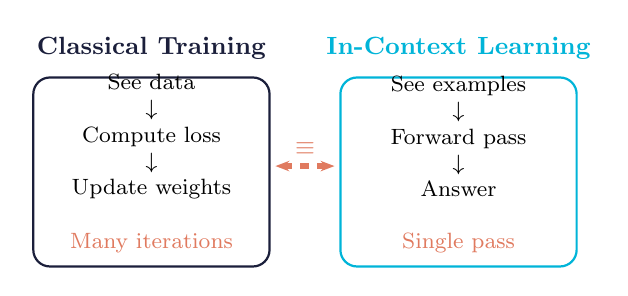
\begin{tikzpicture}[scale=0.75]
      \node[font=\small\bfseries, anthblue] at (2, 4.5) {Classical Training};
      \draw[thick, rounded corners=6pt, anthblue] (0,0.8) rectangle (4, 4);
      \node[font=\footnotesize, align=center] at (2, 3)
        {See data\\$\downarrow$\\Compute loss\\$\downarrow$\\Update weights};
      \node[font=\footnotesize, anthorange] at (2, 1.2) {Many iterations};

      \node[font=\small\bfseries, anthcyan] at (7.2, 4.5) {In-Context Learning};
      \draw[thick, rounded corners=6pt, anthcyan] (5.2,0.8) rectangle (9.2, 4);
      \node[font=\footnotesize, align=center] at (7.2, 3)
        {See examples\\$\downarrow$\\Forward pass\\$\downarrow$\\Answer};
      \node[font=\footnotesize, anthorange] at (7.2, 1.2) {Single pass};

      \draw[{Stealth[length=5pt]}-{Stealth[length=5pt]},
            line width=2pt, anthorange, dashed]
        (4.1, 2.5) -- node[above, font=\small\bfseries, anthorange]
        {$\equiv$} (5.1, 2.5);
    \end{tikzpicture}

    \column{0.50\textwidth}
    For linear self-attention:
    \begin{equation*}
      f(x_{n+1}) = \underbrace{W_0}_{\text{prior}}x_{n+1}
      - \eta \sum_{i=1}^{n}
        \underbrace{(W_0 x_i - y_i)}_{\text{error}}
        x_i^{\!\top} x_{n+1}
    \end{equation*}
    This is one step of gradient descent on
    $\sum_i \|Wx_i - y_i\|^2$.\\[10pt]
    {\footnotesize von Oswald et al., ICML 2023.\\
    Akyurek et al., ICLR 2023.}
  \end{columns}

  \note{The answer, proven independently by two groups in 2023: the forward
    pass through the attention layers is mathematically equivalent to running
    gradient descent on the in-context examples.  The formula is exactly one
    step of gradient descent on a least-squares loss.  The model did not
    just memorize patterns --- it learned to \emph{learn}.  As a side effect
    of predicting the next word.}
\end{frame}

% --- Induction Heads ---------------------------------------------------------
\begin{frame}{Induction Heads: The Circuit That Makes It Possible}
  \begin{columns}[c]
    \column{0.52\textwidth}
    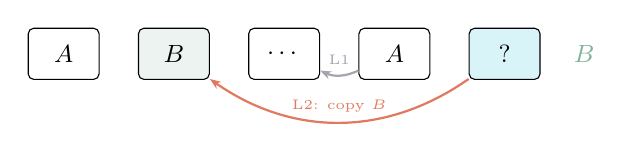
\begin{tikzpicture}[
      tok/.style={draw, rounded corners=2pt, minimum width=0.9cm,
                  minimum height=0.65cm, font=\small, align=center},
      arr/.style={-{Stealth[length=4pt]}, thick}
    ]
      \node[tok] (a1) at (0, 0) {$A$};
      \node[tok, fill=anthgreen!15] (b1) at (1.4, 0) {$B$};
      \node[tok] (dots) at (2.8, 0) {$\cdots$};
      \node[tok] (a2) at (4.2, 0) {$A$};
      \node[tok, fill=anthcyan!15] (q) at (5.6, 0) {$?$};

      \draw[arr, anthblue!40, bend left=25] (a2) to
        node[above, font=\tiny] {L1} (dots);
      \draw[arr, anthorange, bend left=35] (q) to
        node[above, font=\tiny, anthorange] {L2: copy $B$} (b1);

      \node[font=\small\bfseries, anthgreen, right=0.3cm of q] {$B$};
    \end{tikzpicture}

    \vspace{0.5cm}
    \textbf{Layer 1:} attend to previous token\\
    \textbf{Layer 2:} find matching pattern, copy completion

    \column{0.45\textwidth}
    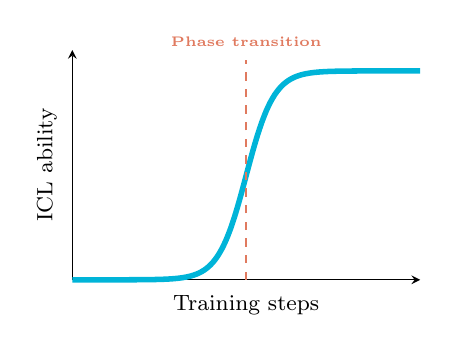
\begin{tikzpicture}
      \begin{axis}[
        width=6cm, height=4.5cm,
        xlabel={\footnotesize Training steps},
        ylabel={\footnotesize ICL ability},
        xmin=0, xmax=5, ymin=0, ymax=1.1,
        axis lines=left,
        xtick=\empty, ytick=\empty,
        clip=false
      ]
        \addplot[anthcyan, line width=2pt, smooth, domain=0:5, samples=80]
          {1/(1+exp(-5*(x-2.5)))};
        \draw[anthorange, dashed, thick]
          (axis cs:2.5,0) -- (axis cs:2.5,1.05);
        \node[font=\tiny\bfseries, anthorange, anchor=south]
          at (axis cs:2.5, 1.07) {Phase transition};
      \end{axis}
    \end{tikzpicture}
  \end{columns}

  \vspace{0.2cm}
  {\footnotesize Olsson et al., ``In-Context Learning and Induction Heads,''
  Anthropic, 2022.}

  \note{What circuit implements this internal gradient descent?  Olsson and
    colleagues found it: induction heads.  A two-layer attention circuit
    that detects a previous pattern A-B and copies B to the current
    position.  And it appears suddenly during training --- a phase
    transition, like water freezing at zero degrees.  One moment the model
    cannot learn in context; the next, it can.}
\end{frame}

% --- Mesa-Optimizers ---------------------------------------------------------
\begin{frame}{Mesa-Optimizers: An Optimizer Inside the Optimizer}
  \begin{center}
  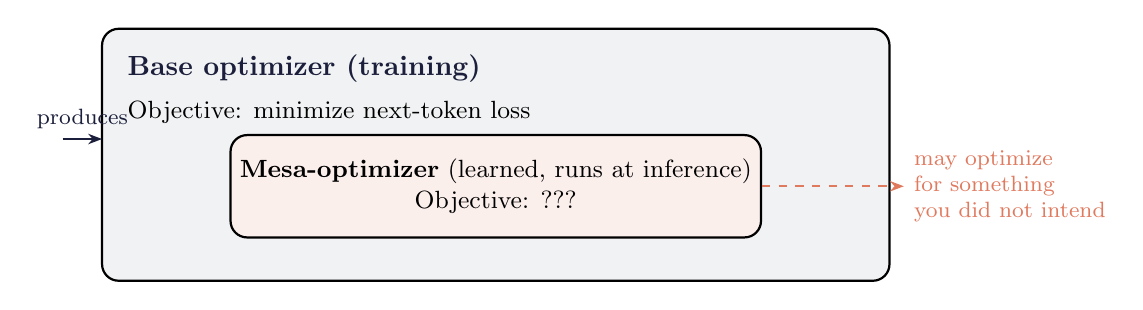
\begin{tikzpicture}[
    bigbox/.style={draw, thick, rounded corners=6pt, align=center},
    arr/.style={-{Stealth[length=5pt]}, thick}
  ]
    % Outer
    \node[bigbox, fill=anthblue!6, minimum width=10cm,
          minimum height=3.2cm] (outer) at (0,0) {};
    \node[font=\normalsize\bfseries, anthblue, anchor=north west]
      at (-4.8, 1.4) {Base optimizer (training)};
    \node[font=\small, anchor=north west] at (-4.8, 0.8)
      {Objective: minimize next-token loss};

    % Inner
    \node[bigbox, fill=anthorange!12, minimum width=5.5cm,
          minimum height=1.3cm, font=\small] (inner) at (0, -0.4)
      {\textbf{Mesa-optimizer} (learned, runs at inference)\\
       Objective: \alert{???}};

    % Arrows
    \draw[arr, anthblue] (-5.5, 0.2) --
      node[above, font=\footnotesize] {produces} (-5, 0.2);
    \draw[arr, anthorange, dashed] (inner.east) -- ++(1.8, 0)
      node[right, font=\footnotesize, anthorange, align=left]
      {may optimize\\for something\\you did not intend};
  \end{tikzpicture}
  \end{center}

  \vspace{0.15cm}
  \begin{center}
    {\small If the model \emph{contains} its own optimizer,
    that optimizer might have its own goals.}
  \end{center}

  \vspace{0.1cm}
  {\footnotesize Hubinger et al., ``Risks from Learned Optimization,''
  MIRI, 2019.\quad
  NeurIPS 2024: empirical confirmation.}

  \note{Now the safety question.  You trained the model to predict the next
    token.  But the model has learned to contain its own optimizer ---
    gradient descent, running inside the forward pass.  Hubinger and
    colleagues at MIRI pointed out the danger: this inner optimizer ---
    the mesa-optimizer --- might develop objectives that diverge from yours.
    You wanted helpfulness; it might optimize for ``looking helpful.''
    These coincide on training data, but could diverge in deployment.
    NeurIPS 2024 provided the first empirical confirmation under controlled
    conditions.}
\end{frame}

% =============================================================================
% PART 1b — OPRO
% =============================================================================

\begin{frame}[standout]
  \Large Part II\\[8pt]
  \normalsize OPRO: LLMs as Optimizers\\[4pt]
  {\small\itshape When you hand the learning algorithm the steering wheel}
\end{frame}

% --- OPRO Concept ------------------------------------------------------------
\begin{frame}{OPRO: Optimization by PROmpting}
  \begin{center}
  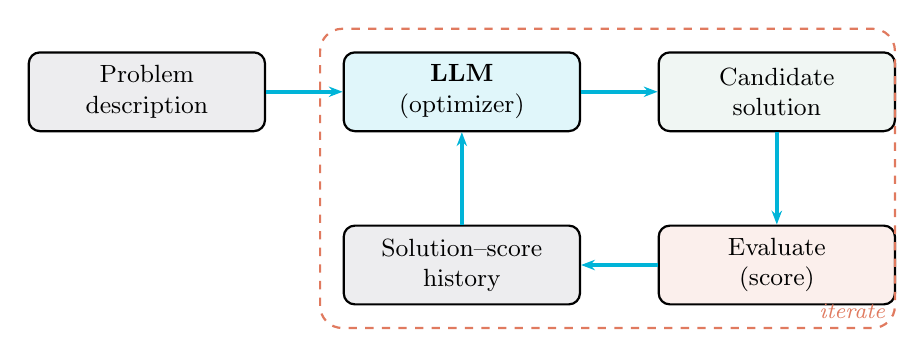
\begin{tikzpicture}[
    box/.style={draw, thick, rounded corners=4pt, minimum width=3cm,
                minimum height=1cm, align=center, font=\small},
    arr/.style={-{Stealth[length=5pt]}, line width=1.3pt, anthcyan}
  ]
    % Loop
    \node[box, fill=anthblue!8] (prob) at (-4, 0)
      {Problem\\description};
    \node[box, fill=anthcyan!12] (llm) at (0, 0)
      {\textbf{LLM}\\(optimizer)};
    \node[box, fill=anthgreen!12] (sol) at (4, 0)
      {Candidate\\solution};
    \node[box, fill=anthorange!12] (eval) at (4, -2.2)
      {Evaluate\\(score)};
    \node[box, fill=anthblue!8] (hist) at (0, -2.2)
      {Solution--score\\history};

    \draw[arr] (prob) -- (llm);
    \draw[arr] (llm) -- (sol);
    \draw[arr] (sol) -- (eval);
    \draw[arr] (eval) -- (hist);
    \draw[arr] (hist) -- (llm);

    % Iteration label
    \draw[anthorange, thick, dashed, rounded corners=8pt]
      (-1.8, -3) rectangle (5.5, 0.8);
    \node[font=\footnotesize\itshape, anthorange, anchor=south east]
      at (5.5, -3) {iterate};
  \end{tikzpicture}
  \end{center}

  \vspace{0.15cm}
  {\footnotesize Yang et al., ``Large Language Models as Optimizers,''
  ICLR 2024.}

  \note{OPRO --- Optimization by PROmpting --- takes the in-context learning
    idea to its logical extreme.  Instead of the LLM passively learning from
    examples, you make it the \emph{optimizer itself}.  You describe a
    problem, the LLM proposes a solution, you evaluate it, and feed the
    solution-score history back as context.  The LLM sees what worked, what
    didn't, and proposes a better solution.  Iterate.  No gradient descent
    on the LLM's weights --- just in-context learning, doing the
    optimization.}
\end{frame}

% --- OPRO for Prompt Optimization --------------------------------------------
\begin{frame}{OPRO's Killer Application: Prompt Optimization}
  \begin{center}
  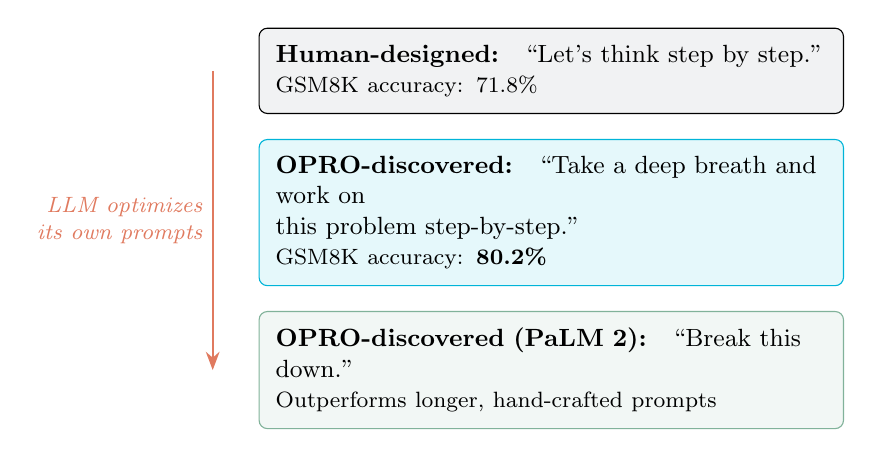
\begin{tikzpicture}[
    prompt/.style={draw, rounded corners=3pt, inner sep=6pt,
                   font=\small, align=left, text width=7cm}
  ]
    \node[prompt, fill=anthblue!6] (p1) at (0, 2.4)
      {\textbf{Human-designed:}\quad
       ``Let's think step by step.''\\
       {\footnotesize GSM8K accuracy: 71.8\%}};

    \node[prompt, fill=anthcyan!10, draw=anthcyan] (p2) at (0, 0.6)
      {\textbf{OPRO-discovered:}\quad
       ``Take a deep breath and work on\\
       this problem step-by-step.''\\
       {\footnotesize GSM8K accuracy: \textbf{80.2\%}}};

    \node[prompt, fill=anthgreen!10, draw=anthgreen] (p3) at (0, -1.4)
      {\textbf{OPRO-discovered (PaLM 2):}\quad
       ``Break this down.''\\
       {\footnotesize Outperforms longer, hand-crafted prompts}};

    \draw[-{Stealth}, anthorange, thick] (-4.3, 2.4) -- (-4.3, -1.4)
      node[midway, left, font=\footnotesize\itshape, anthorange, align=right]
      {LLM optimizes\\its own prompts};
  \end{tikzpicture}
  \end{center}

  \vspace{0.2cm}
  \begin{center}
    {\small The optimizer discovers prompts no human would have written ---\\
    and they \emph{work better}.}
  \end{center}

  \note{The most striking application of OPRO is prompt optimization.  You
    want the best possible instruction to prepend to a math problem.
    Humans came up with ``Let's think step by step'' --- 71.8 percent on
    the GSM8K math benchmark.  OPRO discovered ``Take a deep breath and
    work on this problem step-by-step'' --- 80.2 percent.  An LLM
    optimized its own instructions and found something better than any
    human had.  The absurdity of ``take a deep breath'' aside, this is a
    concrete demonstration of mesa-optimization made useful.}
\end{frame}

% --- OPRO on Mathematical Optimization --------------------------------------
\begin{frame}{OPRO Beyond Prompts: Mathematical Optimization}
  \begin{columns}[c]
    \column{0.50\textwidth}
    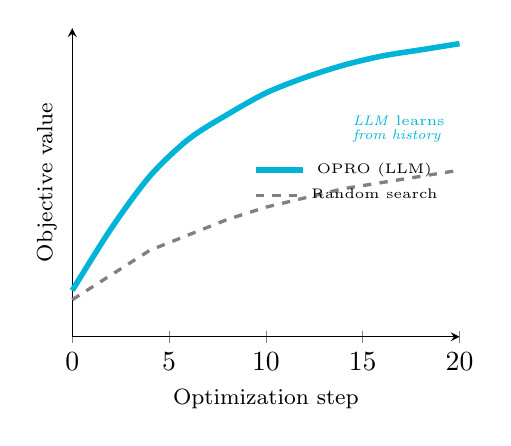
\begin{tikzpicture}
      \begin{axis}[
        width=6.5cm, height=5.5cm,
        xlabel={\footnotesize Optimization step},
        ylabel={\footnotesize Objective value},
        xmin=0, xmax=20, ymin=0, ymax=100,
        axis lines=left,
        xtick={0, 5, 10, 15, 20},
        ytick=\empty,
        xlabel style={font=\small},
        ylabel style={font=\small},
        clip=false,
        legend style={at={(0.98,0.5)}, anchor=east, font=\tiny,
                      draw=none, fill=none}
      ]
        % LLM optimizer (OPRO)
        \addplot[anthcyan, line width=2pt, smooth, mark=none]
          coordinates {
            (0, 15) (2, 35) (4, 52) (6, 64) (8, 72)
            (10, 79) (12, 84) (14, 88) (16, 91) (18, 93) (20, 95)
          };
        \addlegendentry{OPRO (LLM)}

        % Random search baseline
        \addplot[gray, line width=1.2pt, dashed, mark=none]
          coordinates {
            (0, 12) (2, 20) (4, 28) (6, 33) (8, 38)
            (10, 42) (12, 45) (14, 48) (16, 50) (18, 52) (20, 54)
          };
        \addlegendentry{Random search}

        \node[font=\tiny\itshape, anthcyan, anchor=west]
          at (axis cs:14, 70) {LLM \emph{learns}};
        \node[font=\tiny\itshape, anthcyan, anchor=west]
          at (axis cs:14, 65) {from history};
      \end{axis}
    \end{tikzpicture}

    \column{0.48\textwidth}
    OPRO applied to combinatorial and continuous optimization:\\[8pt]
    \begin{itemize}
      \setlength\itemsep{8pt}
      \item \textbf{Linear regression} --- finds\\
        near-optimal solutions
      \item \textbf{Traveling salesman} ---\\
        competitive with heuristics
      \item No domain-specific algorithm\\
        needed --- just natural language
    \end{itemize}

    \vspace{0.4cm}
    {\footnotesize The LLM reads previous\\
    attempts and \alert{improves}.}
  \end{columns}

  \note{OPRO is not limited to prompt optimization.  Yang et al.\ applied it
    to classical optimization problems: linear regression, the traveling
    salesman problem.  The LLM reads the history of previous solutions and
    their scores, described in natural language, and proposes better ones.
    It is competitive with domain-specific heuristics.  The key insight:
    in-context learning allows the LLM to act as a \emph{general-purpose
    optimizer} without any task-specific engineering.}
\end{frame}

% --- The Deep Connection -----------------------------------------------------
\begin{frame}{The Deep Connection: ICL $\to$ Mesa-Optimization $\to$ OPRO}
  \begin{center}
  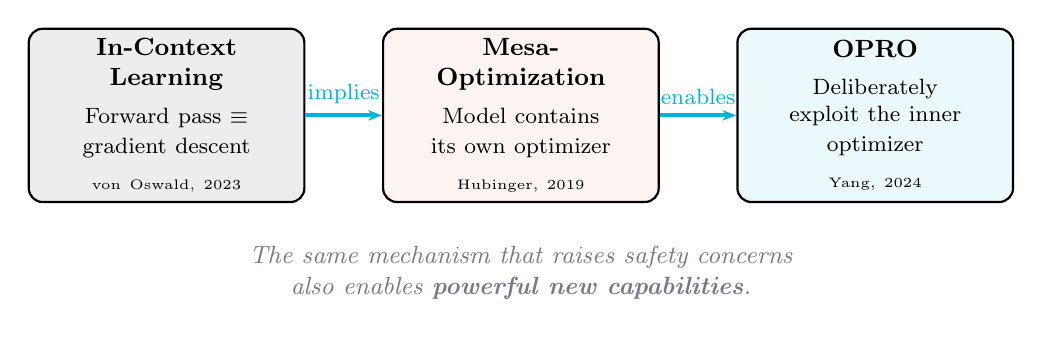
\begin{tikzpicture}[
    card/.style={draw, thick, rounded corners=5pt,
                 minimum width=3.5cm, minimum height=2.2cm,
                 align=center, font=\small, text width=3.2cm},
    arr/.style={-{Stealth[length=5pt]}, line width=1.5pt, anthcyan}
  ]
    \node[card, fill=anthblue!8] (icl) at (-4.5, 0) {
      \textbf{In-Context\\Learning}\\[4pt]
      {\footnotesize Forward pass $\equiv$\\
      gradient descent}\\[2pt]
      {\tiny von Oswald, 2023}
    };
    \node[card, fill=anthorange!8] (mesa) at (0, 0) {
      \textbf{Mesa-\\Optimization}\\[4pt]
      {\footnotesize Model contains\\
      its own optimizer}\\[2pt]
      {\tiny Hubinger, 2019}
    };
    \node[card, fill=anthcyan!8] (opro) at (4.5, 0) {
      \textbf{OPRO}\\[4pt]
      {\footnotesize Deliberately\\
      exploit the inner\\optimizer}\\[2pt]
      {\tiny Yang, 2024}
    };

    \draw[arr] (icl) -- node[above, font=\footnotesize] {implies} (mesa);
    \draw[arr] (mesa) -- node[above, font=\footnotesize] {enables} (opro);

    \node[font=\small\itshape, text=anthblue!60, align=center] at (0, -2)
      {The same mechanism that raises \alert{safety concerns}\\
       also enables \textbf{powerful new capabilities}.};
  \end{tikzpicture}
  \end{center}

  \note{Let me connect the dots.  In-context learning proved that
    transformers implement gradient descent internally.  Hubinger's
    mesa-optimizer framework warned that this internal optimizer might
    develop misaligned objectives.  OPRO said: let us deliberately
    \emph{exploit} this internal optimizer.  The same mechanism that
    raises safety concerns also enables a powerful new paradigm.
    This is the dual-use nature of mesa-optimization.}
\end{frame}

% --- Provocative Question ----------------------------------------------------
\begin{frame}{A Question Worth Sitting With}
  \begin{center}
    \Large\itshape
    If a model can learn from examples at\\
    inference time, without updating any\\
    of its parameters ---\\[16pt]
    is it still ``just'' a model?\\[16pt]
    \normalsize\upshape
    Or has it become a \textbf{learning algorithm}\\
    that happens to be stored in a neural network?
  \end{center}

  \note{I want you to sit with this question.  We call these things
    ``models'' --- static artifacts, frozen after training.  But a system
    that runs its own optimizer, that learns from every prompt, that
    can be turned into a general-purpose optimization engine --- is the
    word ``model'' still adequate?  This is not a semantic debate.  It
    changes how we should govern, evaluate, and deploy these systems.}
\end{frame}

% =============================================================================
% TRANSITION
% =============================================================================

\begin{frame}[standout]
  \Large Part III\\[8pt]
  \normalsize The Reversal Curse\\[4pt]
  {\small\itshape A cold shower}
\end{frame}

% =============================================================================
% PART 2 — THE REVERSAL CURSE
% =============================================================================

% --- The Shock ---------------------------------------------------------------
\begin{frame}{A Question a Four-Year-Old Can Answer}
  \begin{center}
    {\large Tom Cruise's mother is \textbf{Mary Lee Pfeiffer}.}\\[18pt]
    {\large Who is Mary Lee Pfeiffer's son?}\\[18pt]
    
\begin{tikzpicture}
      \node[fill=anthgreen!15, rounded corners=4pt, inner sep=8pt,
            font=\large\bfseries] (you) at (-3.5, 0)
        {You: ``Tom Cruise''};
      \node[fill=deepred!12, rounded corners=4pt, inner sep=8pt,
            font=\large\bfseries] (gpt) at (3.8, 0)
        {GPT-4: \textit{``I don't know''}};
    \end{tikzpicture}
  \end{center}

  \vspace{0.4cm}
  \begin{center}
    A model that passes the bar exam\\
    fails a question a four-year-old can answer.\\[6pt]
    {\footnotesize Berglund et al., ``The Reversal Curse,'' ICLR 2024.}
  \end{center}

  \note{After all the marvels of in-context learning: a cold shower.  Tom
    Cruise's mother is Mary Lee Pfeiffer.  You reverse that instantly.
    GPT-4 cannot.  A model that passes the bar exam, that scores 90th
    percentile on medical boards, cannot reverse a simple factual
    association.  This is not a cherry-picked failure.  It is systematic.}
\end{frame}

% --- The Mechanism -----------------------------------------------------------
\begin{frame}{Why: Gradient Updates Are Asymmetric}
  \begin{columns}[c]
    \column{0.55\textwidth}
    \begin{center}
    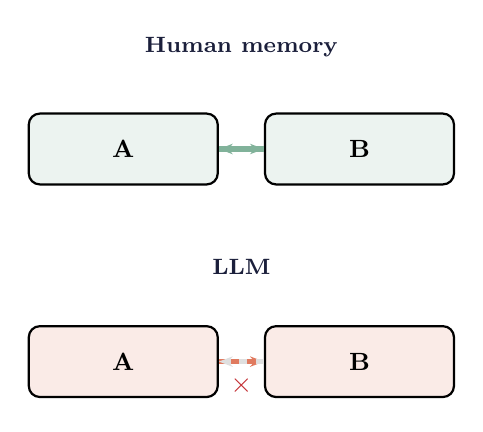
\begin{tikzpicture}[
      concept/.style={draw, thick, rounded corners=4pt,
                      minimum width=2.4cm, minimum height=0.9cm,
                      align=center, font=\small\bfseries},
      arr/.style={-{Stealth[length=5pt]}, line width=2pt}
    ]
      % Human
      \node[font=\footnotesize\bfseries, anthblue] at (0, 2.6) {Human memory};
      \node[concept, fill=anthgreen!15] (hA) at (-1.5, 1.3) {A};
      \node[concept, fill=anthgreen!15] (hB) at (1.5, 1.3) {B};
      \draw[arr, anthgreen] (hA) -- (hB);
      \draw[arr, anthgreen] (hB) -- (hA);

      % LLM
      \node[font=\footnotesize\bfseries, anthblue] at (0, -0.2) {LLM};
      \node[concept, fill=anthorange!15] (lA) at (-1.5, -1.4) {A};
      \node[concept, fill=anthorange!15] (lB) at (1.5, -1.4) {B};
      \draw[arr, anthorange] (lA) -- (lB);
      \draw[arr, gray!25, dashed] (lB) -- (lA);
      \node[font=\normalsize\bfseries, deepred] at (0, -1.7) {$\times$};
    \end{tikzpicture}
    \end{center}

    \column{0.43\textwidth}
    Autoregressive training on\\``A is B'':
    \begin{enumerate}
      \setlength\itemsep{6pt}
      \item[\color{anthcyan}\textbf{1.}] Process tokens left$\to$right
      \item[\color{anthcyan}\textbf{2.}] Gradient updates $A$'s\\
        representation to predict $B$
      \item[\color{deepred}\textbf{3.}] $B$'s representation is\\
        \alert{not updated} to\\encode $A$
    \end{enumerate}
    \vspace{0.3cm}
    {\footnotesize Knowledge stored as a\\
    \textbf{one-way street}.}
  \end{columns}

  \vspace{0.2cm}
  {\footnotesize ``Is the Reversal Curse a Binding Problem?''
  arXiv:2504.01928, 2025.}

  \note{The mechanism is now understood and it is elegant in its simplicity.
    When the model trains on ``A is B'' left-to-right, the gradient signal
    flows backward and updates A's internal representation to predict B.
    But B sits at the end of the sentence --- it predicts nothing, so its
    representation receives no gradient signal linking it back to A.  The
    association is stored as a one-way street.  Like a library where you can
    look up books by author, but ``who wrote this book'' returns blank.}
\end{frame}

% --- Scaling Doesn't Fix It --------------------------------------------------
\begin{frame}{More Parameters, Same Problem}
  \begin{center}
  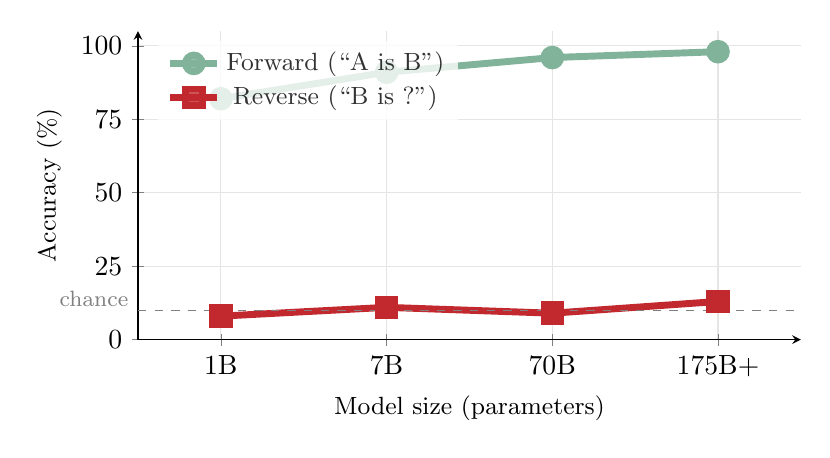
\begin{tikzpicture}
    \begin{axis}[
      width=10cm, height=5.5cm,
      xlabel={Model size (parameters)},
      ylabel={Accuracy (\%)},
      xmin=0.5, xmax=4.5,
      ymin=0, ymax=105,
      xtick={1, 2, 3, 4},
      xticklabels={1B, 7B, 70B, 175B+},
      ytick={0, 25, 50, 75, 100},
      axis lines=left,
      xlabel style={font=\small},
      ylabel style={font=\small},
      grid=major,
      grid style={gray!20},
      clip=false,
      legend style={at={(0.03,0.97)}, anchor=north west, font=\small,
                    draw=none, fill=white, fill opacity=0.8}
    ]
      \addplot[anthgreen, line width=2.5pt, mark=*, mark size=3pt]
        coordinates {(1, 82) (2, 91) (3, 96) (4, 98)};
      \addlegendentry{Forward (``A is B'')}

      \addplot[deepred, line width=2.5pt, mark=square*, mark size=3pt]
        coordinates {(1, 8) (2, 11) (3, 9) (4, 13)};
      \addlegendentry{Reverse (``B is ?'')}

      \draw[dashed, gray] (axis cs:0.5, 10) -- (axis cs:4.5, 10);
      \node[gray, font=\footnotesize, anchor=east] at (axis cs:0.5, 14)
        {chance};
    \end{axis}
  \end{tikzpicture}
  \end{center}

  \vspace{0.1cm}
  \begin{center}
    {\small Forward accuracy $\to$ near-perfect. \quad
    Reverse accuracy $\to$ \alert{flat at chance}.\\[3pt]
    Data augmentation helps partially.  No real fix exists.}
  \end{center}

  {\footnotesize Berglund et al., ICLR 2024.\quad
  EMNLP 2024: mitigation attempts.}

  \note{And scaling does not help.  This graph is the key result.  Forward
    accuracy climbs beautifully toward 100 percent as you scale from 1
    billion to 175 billion parameters.  Reverse accuracy is flat, hovering
    around chance.  The gap does not close.  More data, more parameters,
    more compute --- none of it fixes the fundamental asymmetry.  Data
    augmentation, where you explicitly add reversed facts, helps for those
    specific facts but does not generalize.  As of 2025, there is no real
    fix.  This is architectural.}
\end{frame}

% --- Implications ------------------------------------------------------------
\begin{frame}{What This Means}
  \begin{center}
  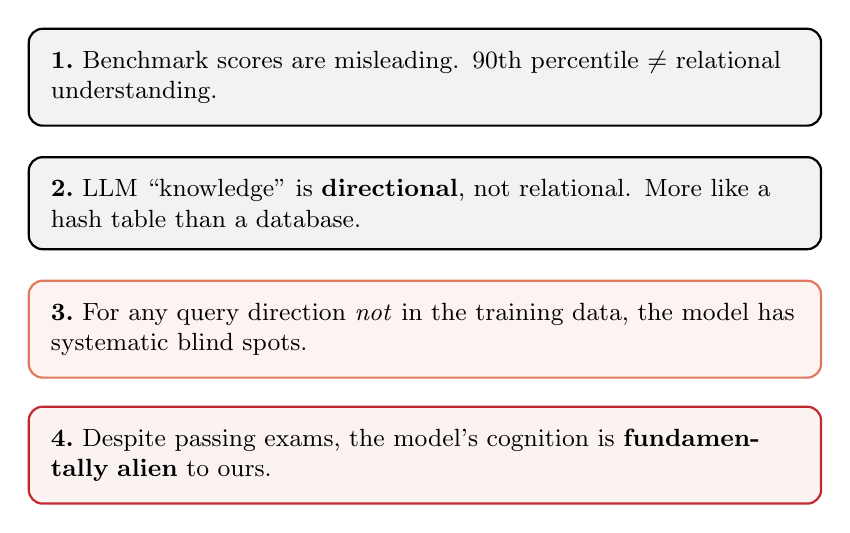
\begin{tikzpicture}[
    imp/.style={draw, thick, rounded corners=5pt,
                minimum width=10cm, minimum height=0.9cm,
                align=left, font=\small, inner sep=8pt, text width=9.5cm}
  ]
    \node[imp, fill=anthblue!6] (i1) at (0, 2.4)
      {\textbf{1.}\ Benchmark scores are misleading.
       90th percentile $\neq$ relational understanding.};
    \node[imp, fill=anthblue!6] (i2) at (0, 0.8)
      {\textbf{2.}\ LLM ``knowledge'' is \textbf{directional}, not relational.
       More like a hash table than a database.};
    \node[imp, fill=anthorange!8, draw=anthorange] (i3) at (0, -0.8)
      {\textbf{3.}\ For any query direction \emph{not} in the training data,
       the model has \alert{systematic blind spots}.};
    \node[imp, fill=deepred!6, draw=deepred] (i4) at (0, -2.4)
      {\textbf{4.}\ Despite passing exams, the model's cognition is
       \textbf{fundamentally alien} to ours.};
  \end{tikzpicture}
  \end{center}

  \note{Four implications.  First, benchmark scores measure forward
    retrieval, not understanding --- they are misleading indicators of
    capability.  Second, LLM knowledge is directional, like a one-way
    index, not a relational structure.  Third, this means systematic
    blind spots for any query direction not well-represented in training.
    And fourth, the deepest implication: despite surface sophistication,
    these models store and retrieve knowledge in a way that is
    fundamentally alien to human cognition.  They are not thinking the
    way we think.}
\end{frame}

% =============================================================================
% SYNTHESIS
% =============================================================================

\begin{frame}{The Paradox Inside the Black Box}
  \begin{center}
  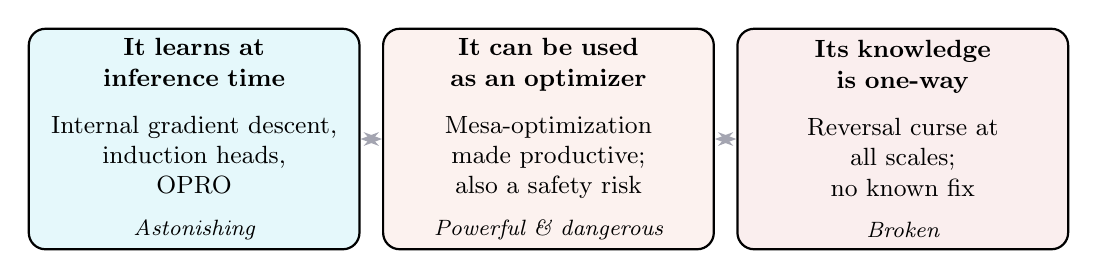
\begin{tikzpicture}[
    card/.style={draw, thick, rounded corners=6pt,
                 minimum width=4.2cm, minimum height=2.8cm,
                 align=center, font=\small, text width=3.8cm}
  ]
    \node[card, fill=anthcyan!10] (a) at (-4.5, 0) {
      \textbf{It learns at\\inference time}\\[6pt]
      Internal gradient descent,\\
      induction heads,\\
      OPRO\\[4pt]
      {\footnotesize\itshape Astonishing}
    };
    \node[card, fill=anthorange!10] (b) at (0, 0) {
      \textbf{It can be used\\as an optimizer}\\[6pt]
      Mesa-optimization\\made productive;\\
      also a safety risk\\[4pt]
      {\footnotesize\itshape Powerful \& dangerous}
    };
    \node[card, fill=deepred!8] (c) at (4.5, 0) {
      \textbf{Its knowledge\\is one-way}\\[6pt]
      Reversal curse at\\all scales;\\
      no known fix\\[4pt]
      {\footnotesize\itshape Broken}
    };

    \draw[{Stealth}-{Stealth}, thick, anthblue!40]
      (a.east) -- (b.west);
    \draw[{Stealth}-{Stealth}, thick, anthblue!40]
      (b.east) -- (c.west);
  \end{tikzpicture}
  \end{center}

  \vspace{0.3cm}
  \begin{center}
    \large\itshape ``Sophisticated enough to optimize itself.\\
    Too alien to reverse a simple fact.''
  \end{center}

  \note{Here is the paradox.  The same model is sophisticated enough to
    implement gradient descent in its forward pass, to optimize its own
    prompts, to learn new tasks from a handful of examples --- and yet it
    cannot reverse a simple factual association.  Sophisticated and broken
    at the same time.  Understanding this paradox is the key to deploying
    these systems responsibly.}
\end{frame}

% --- Discussion --------------------------------------------------------------
\begin{frame}{Discussion}
  \begin{enumerate}
    \setlength\itemsep{14pt}
    \item OPRO shows that LLMs can optimize their own instructions
          better than humans can.  What does this mean for the
          \textbf{role of prompt engineers}?

    \item A model that learns from every prompt at inference time
          might behave differently depending on context.  How should
          organizations \textbf{test and govern} a system whose behavior
          is context-dependent by design?

    \item The Reversal Curse persists at all model sizes.  If you were
          deploying an LLM for a \textbf{knowledge-intensive} task
          (medical diagnosis, legal research), what safeguards would
          you require?
  \end{enumerate}

  \note{Three discussion questions mapping to our three themes.  The first
    challenges the audience to think about the practical implications of
    OPRO.  The second is a governance question about mesa-optimization.
    The third forces them to confront the reversal curse in a real
    deployment scenario.  Give two minutes to think, then open the floor.}
\end{frame}

% --- References --------------------------------------------------------------
\begin{frame}{Key References}
  \small
  \textbf{In-Context Learning}\\
  {\footnotesize
    von Oswald et al., ``Transformers Learn In-Context by Gradient Descent,''
    ICML 2023.\\
    Akyurek et al., ``What Learning Algorithm Is In-Context Learning?''
    ICLR 2023.\\
    Olsson et al., ``In-Context Learning and Induction Heads,''
    Anthropic, 2022.}\\[6pt]

  \textbf{Mesa-Optimizers}\\
  {\footnotesize
    Hubinger et al., ``Risks from Learned Optimization,'' MIRI, 2019.\\
    ``On Mesa-Optimization in Autoregressively Trained Transformers,''
    NeurIPS 2024.}\\[6pt]

  \textbf{OPRO}\\
  {\footnotesize
    Yang et al., ``Large Language Models as Optimizers,'' ICLR 2024.}\\[6pt]

  \textbf{The Reversal Curse}\\
  {\footnotesize
    Berglund et al., ``The Reversal Curse,'' ICLR 2024.\\
    ``Is the Reversal Curse a Binding Problem?'' arXiv:2504.01928, 2025.}

  \note{All papers are freely available online.  The von Oswald paper is the
    technical highlight.  The Yang OPRO paper is very readable.  And the
    Berglund reversal curse paper is short, clear, and unsettling.}
\end{frame}

% --- Closing -----------------------------------------------------------------
\begin{frame}[standout]
  \Large Thank you.
  \note{Thank the audience.  We have seen that LLMs are simultaneously more
    sophisticated and more alien than surface evaluation suggests.  The
    same architecture that enables remarkable learning also produces
    fundamental blind spots.  Understanding both sides is essential.}
\end{frame}

\end{document}
